%%% Template originaly created by Karol Kozioł (mail@karol-koziol.net) and modified for ShareLaTeX use

\documentclass[a4paper,11pt]{article}

\usepackage[T1]{fontenc}
\usepackage[utf8]{inputenc}
\usepackage{graphicx}
\usepackage{xcolor}
\usepackage[export]{adjustbox}
\usepackage{titlesec}
\usepackage{sectsty}
\allsectionsfont{\sffamily}

\usepackage{tgheros}
\usepackage[defaultmono]{droidmono}
\usepackage{mathptmx}

\usepackage{amsmath,amssymb,amsthm,textcomp}
\usepackage{enumerate}
\usepackage{multicol}
\usepackage{tikz}
\usepackage{tabto}
\usepackage{pxfonts}
\usepackage{geometry}
\geometry{left=25mm,right=25mm,%
bindingoffset=0mm, top=20mm,bottom=20mm}


\linespread{1.2}

\newcommand{\linia}{\rule{\linewidth}{0.5pt}}

% custom theorems if needed
\newtheoremstyle{mytheor}
    {1ex}{1ex}{\normalfont}{0pt}{\scshape}{.}{1ex}
    {{\thmname{#1 }}{\thmnumber{#2}}{\thmnote{ (#3)}}}

\theoremstyle{mytheor}
\newtheorem{defi}{Definition}
\newtheoremstyle{mytheor}
    {1ex}{1ex}{\normalfont}{0pt}{\scshape}{.}{1ex}
    {{\thmname{#1 }}{}{\thmnote{ (#3)}}}

\theoremstyle{mytheor}
\newtheorem{nb}{Please Note}
% my own titles
\makeatletter
\renewcommand{\maketitle}{
\begin{center}
\vspace{2ex}
{\huge \textsf{\textbf{\@title}}}
\vspace{1ex}
\\
\linia\\
\textsf{\@date \hfill
\@author}
\vspace{4ex}
\end{center}
}
\makeatother
%%%

% custom footers and headers
\usepackage{fancyhdr}
\pagestyle{fancy}
\lhead{}
\chead{}
\rhead{}
\lfoot{Assignment 2}
\cfoot{}
\rfoot{Page \thepage}
\renewcommand{\headrulewidth}{0pt}
\renewcommand{\footrulewidth}{0pt}
%

% code listing settings
\usepackage{listings}
\usepackage[space=true]{accsupp}

\definecolor{codegreen}{rgb}{0,0.6,0}
\definecolor{codegray}{rgb}{0.5,0.5,0.5}
\definecolor{inlinecode}{rgb}{0.1,0.1,0.1}
\definecolor{codepurple}{rgb}{0.58,0,0.82}
\definecolor{backcolour}{rgb}{0.95,0.95,0.92}
\lstset{
    language=C,
    basicstyle=\ttfamily\small,
    aboveskip={1.0\baselineskip},
    breakatwhitespace=false,         
    keepspaces=true,
    belowskip={1.0\baselineskip},
    columns=fullflexible,
    extendedchars=true,
    breaklines=true,
    tabsize=4,
    frame=lines,
    showtabs=false,
    showspaces=false,
    showstringspaces=false,
    commentstyle=\color{codegray},
    keywordstyle=\bfseries,
%    stringstyle=\color{codegreen},
    numbers=left,
    numberstyle=\color{codegray}\footnotesize\noncopynumber,
    stepnumber=1,
    numbersep=10pt,
    captionpos=t,
    escapeinside={\%*}{*)},
}

\newcommand{\noncopynumber}[1]{
    \BeginAccSupp{method=escape,ActualText={}}
    #1
    \EndAccSupp{}
}

%%%----------%%%----------%%%----------%%%----------%%%

\begin{document}

\title{CSE-016 Programming Lab Assignment \textnumero{} 2}

\date{16/03/2024}

\author{Youssef Ahmed Samy Kassem\\ \hfill ID 9545 -- Group 3 -- Lab 1\\ \hfill SSP -- Faculty of Engineering, Alexandria University\\}

\maketitle
\textsf{\textsl{Document structure is detailed in the second page.\\\textbf{Solutions begin from the third page.}}}
\section{Problems}
\subsection{Problem (1)}
John is responsible for planting the street with trees; he can give you the length of the street in
meters, the distance between each two trees in a meter, and the cost of planting each tree in
dollars. Write a program that should read this information and then print the number of trees
needed and the total cost.
\subsection{Problem (2)}
Write a program that calculates the squares, cubes, square root, and exponent ($e^{x}$) of the
numbers from 0 to 5 and uses tabs to print the following table of values:\\\\
\setlength{\tabcolsep}{18pt}
\begin{tabular}{ l l l l l }
Number & Square & Cube & Root & Exponent \\ 
 0 & 0  & 0 & 0.0 & 1.0 \\  
 .. & .. & .. & .. & .. \\
 .. & .. & .. & .. & ..
\end{tabular}
\newpage
\tableofcontents
\newpage
\section{Solutions}
\subsection{Solution to Problem (1)}
\subsubsection{Source Code}
\begin{lstlisting}[escapechar=\^,label={list:first},title=Program's \texttt{\color{inlinecode}{main.c}} File -- console input/output-oriented application to solve the problem]
#include <math.h>
#include <stdio.h>

int main() {
  // Runtime variable declarations
  float streetlen, treedist, treecost, totalcost;
  int treenum;

  // Input prompts
  printf("Hello, John! Let's help you fill the street with trees.\n\n");
  printf("Please enter the length of the street (m): ");
  scanf("%f", &streetlen);
  printf("Now enter the distance you want between each tree (m): ");
  scanf("%f", &treedist);
  printf("Great! Finally, enter the cost of planting one tree ($): ");
  scanf("%f", &treecost);
  printf("\n"); // To separate input from results

  // Calculations
  treenum = 1 + floor(streetlen / treedist);
  totalcost = (float) treecost * treenum;

  // Outputting the results
  printf("You will have to plant %d tree(s)\n", treenum);
  printf("The total price you'll pay will be $%.2f\n", totalcost);

  return 0;
}
\end{lstlisting}
\newpage
\subsubsection{Outcome}
\paragraph{Test Input Samples\\}

\begin{tabular}{ l l l l }
\# & Street Length & Distance Btn. Trees & Cost/ Tree\\
(1) & 100 & 10 & 12\\
(2) & 987 & 10 & 13.98\\
\end{tabular}
\subparagraph{Obtained Results}

\begin{tabular}{ l l l }
\# & Number of Trees & Total Cost\\
(1) & 11 & 132.00 \\
(2) & 99 & 1384.02 \\
\end{tabular}
\\\\The obtained results match the expected results.
\paragraph{Console Output}
\begin{lstlisting}[escapechar=\%,language=tex,numbers=none,label={list:second},title=Program's output to console in plaintext -- using inputs from test sample (1)]
Hello, John! Let's help you fill the street with trees.

Please enter the length of the street (m): 100
Now enter the distance you want between each tree (m): 10
Great! Finally, enter the cost of planting one tree ($): 12

You will have to plant 11 tree(s)
The total price you'll pay will be $132.00
%
\end{lstlisting}
\begin{center}
\textit{\\\ \\\ \\\ \\\ \\\ \\\ \\\ \\Turn over the page for the solution to problem (2)}
\end{center}
\newpage
\subsection{Solution to Problem (2)}
\subsubsection{Source Code}
\begin{lstlisting}[label={list:third},title=Program's \texttt{\color{inlinecode}{main.c}} File -- console application to output the full table as described in the problem]
#include <math.h>
#include <stdio.h>

int main() {
  printf("Number\tSquare\tCube\tRoot\tExponent\n");
  printf("0\t%d\t%d\t%.1f\t%.1f\n",((int)pow(0,2)),((int)pow(0,3)),sqrt(0),exp(0));
  printf("1\t%d\t%d\t%.1f\t%.1f\n",((int)pow(1,2)),((int)pow(1,3)),sqrt(1),exp(1));
  printf("2\t%d\t%d\t%.1f\t%.1f\n",((int)pow(2,2)),((int)pow(2,3)),sqrt(2),exp(2));
  printf("3\t%d\t%d\t%.1f\t%.1f\n",((int)pow(3,2)),((int)pow(3,3)),sqrt(3),exp(3));
  printf("4\t%d\t%d\t%.1f\t%.1f\n",((int)pow(4,2)),((int)pow(4,3)),sqrt(4),exp(4));
  printf("5\t%d\t%d\t%.1f\t%.1f\n",((int)pow(5,2)),((int)pow(5,3)),sqrt(5),exp(5));
  return 0;
}
\end{lstlisting}
\textsl{Please note that the line numbers are purely for readability purposes and are not part of the code.\\Please also note that on lines where there is no new line number, there is \textbf{NO} actual line break in the code and that this is meant to be read as one single line.}
\subsubsection{Outcome}
\paragraph{Console Output}
\begin{lstlisting}[escapechar=\%,language=tex,numbers=none,label={list:fourth},title=Program's output to console in plaintext]
Number	Square	Cube	Root	Exponent
0		0		0		0.0		1.0
1		1		1		1.0		2.7
2		4		8		1.4		7.4
3		9		27		1.7		20.1
4		16		64		2.0		54.6
5		25		125		2.2		148.4
%
\end{lstlisting}
\subsection{Evidence of Work (Screenshots)}
\subsubsection{Problem (1) Screenshots}
\subparagraph{Close Up Source-code Screenshot\\}
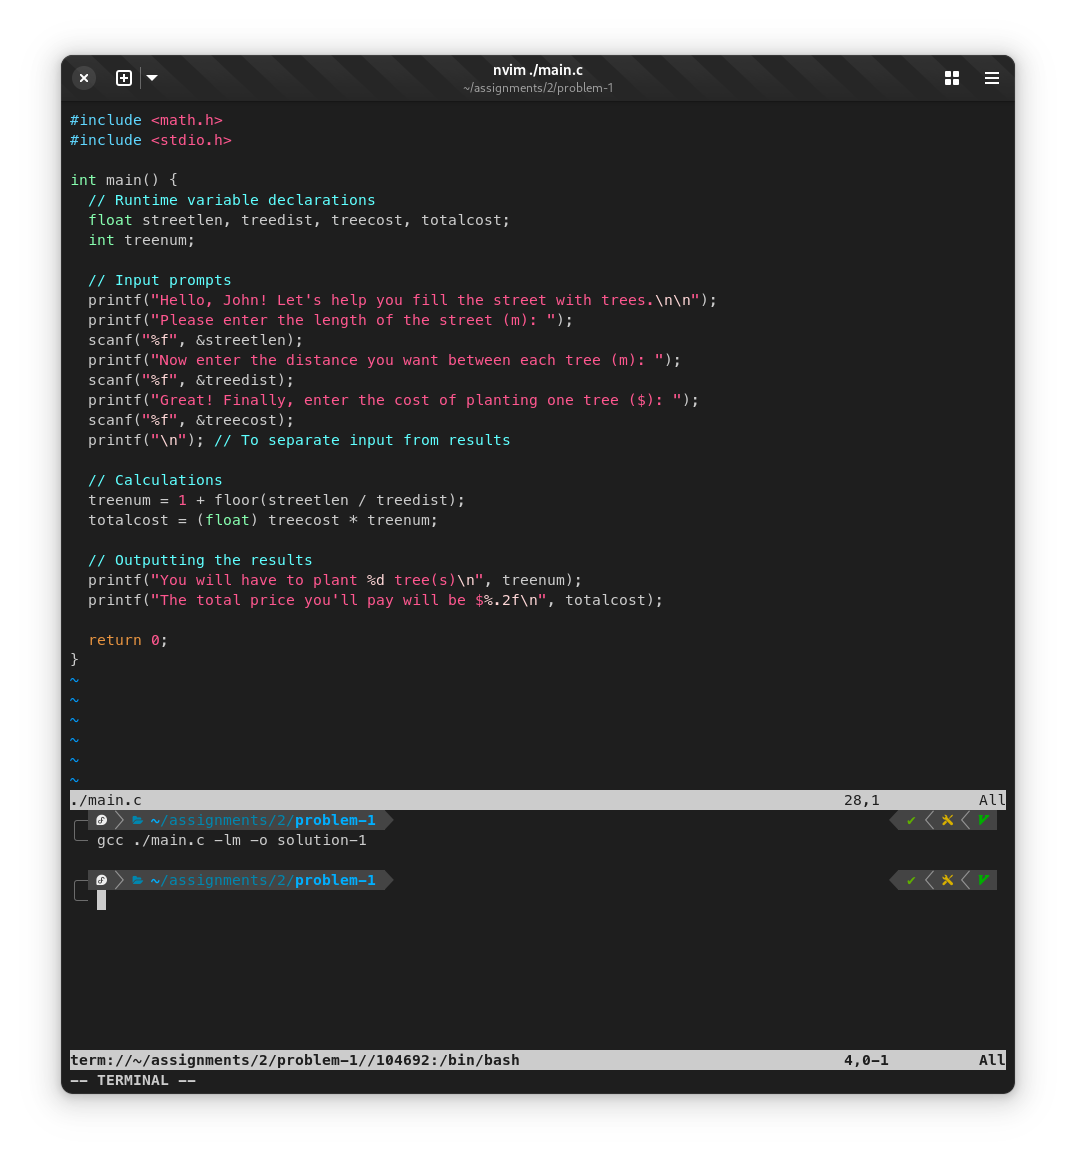
\includegraphics[width=1\linewidth,center]{src-1.png}
\subparagraph{Close Up Output Console Screenshot\\}
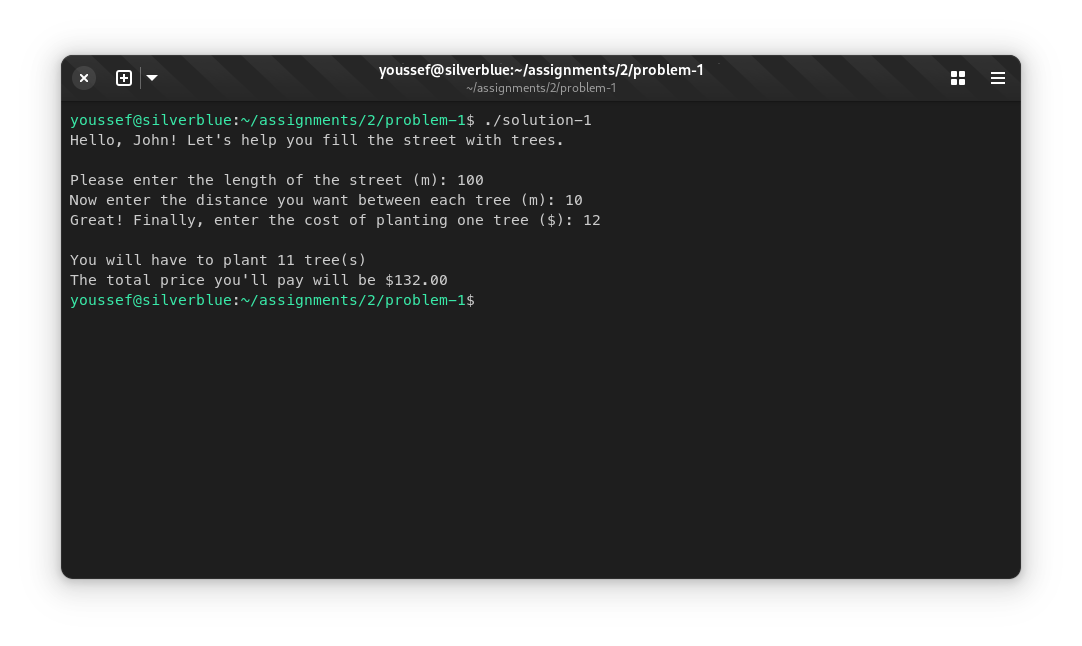
\includegraphics[width=1\linewidth,center]{out-1.png}
\subparagraph{Linux Desktop Screenshot\\\\}
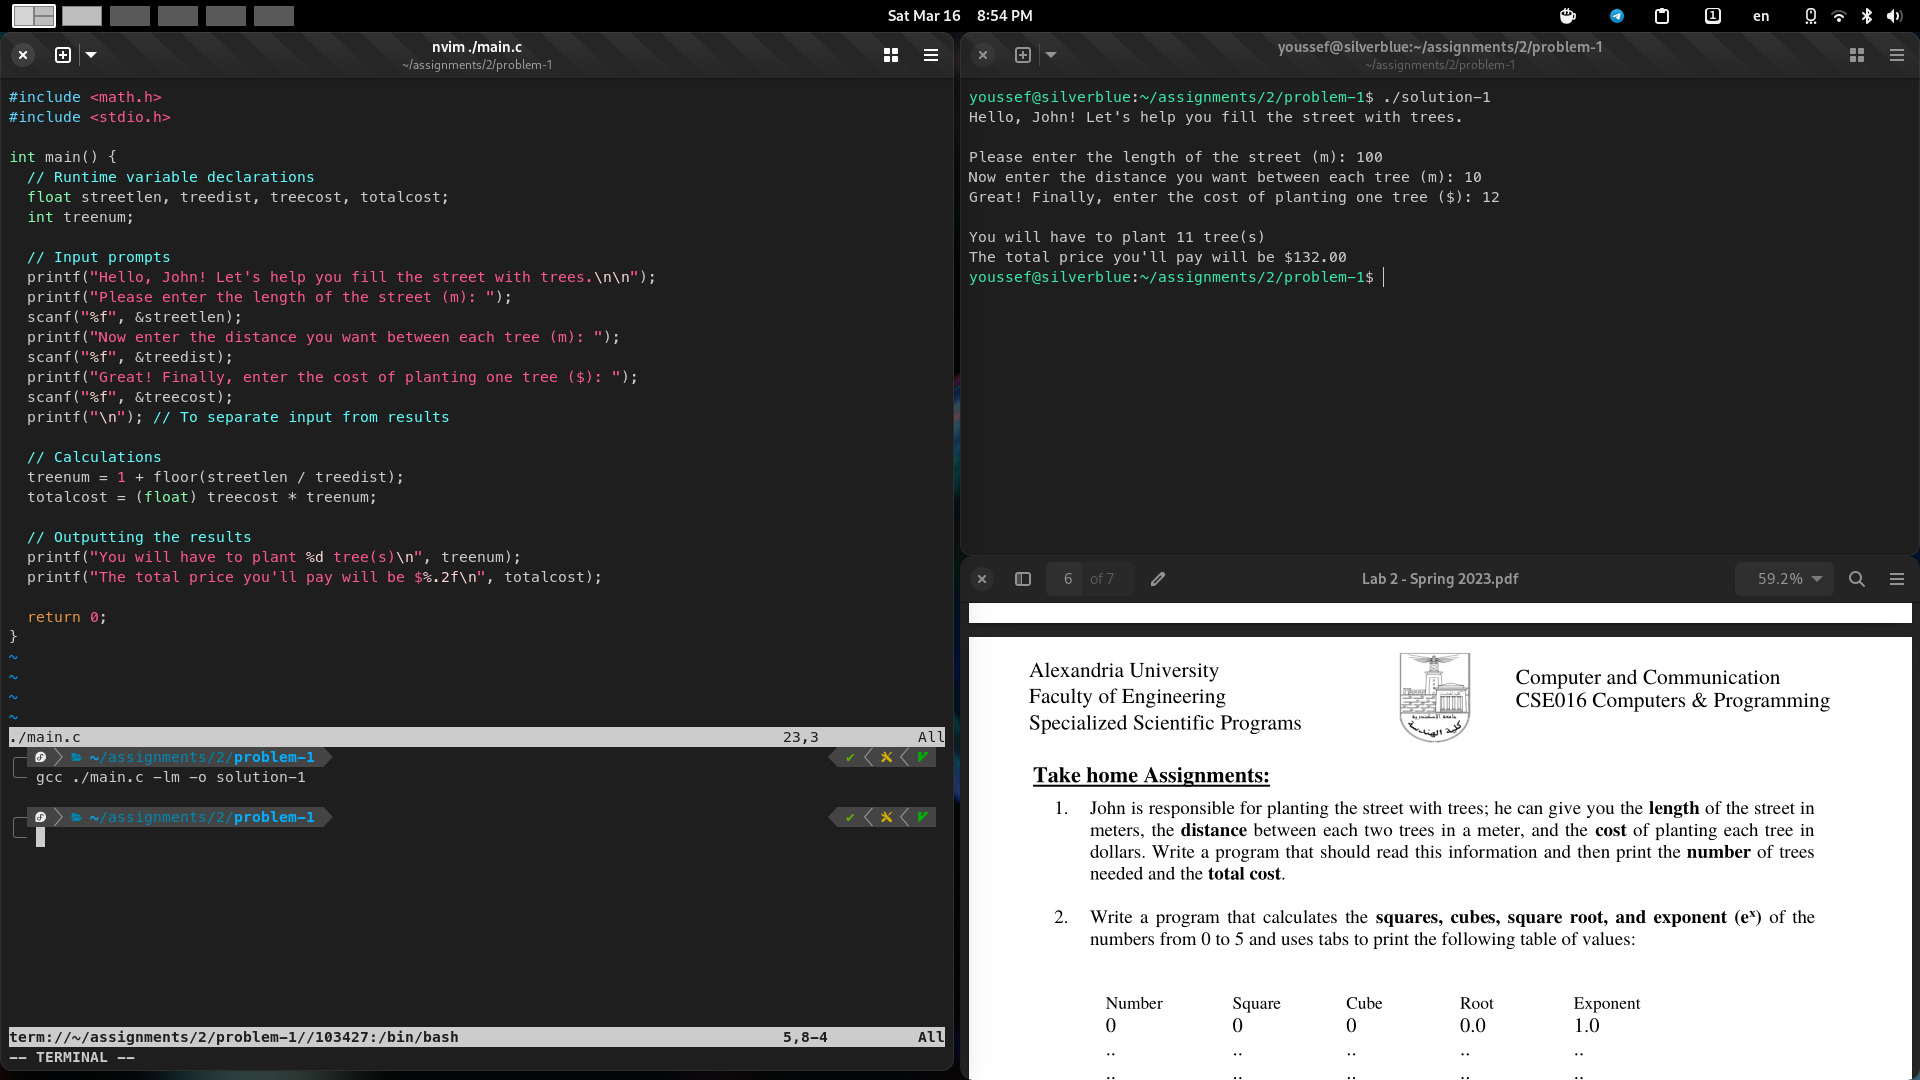
\includegraphics[width=1\linewidth,center]{desktop-1.png}
\newpage
\subsubsection{Problem (2) Screenshots}
\subparagraph{Close Up Source-code Screenshot\\}
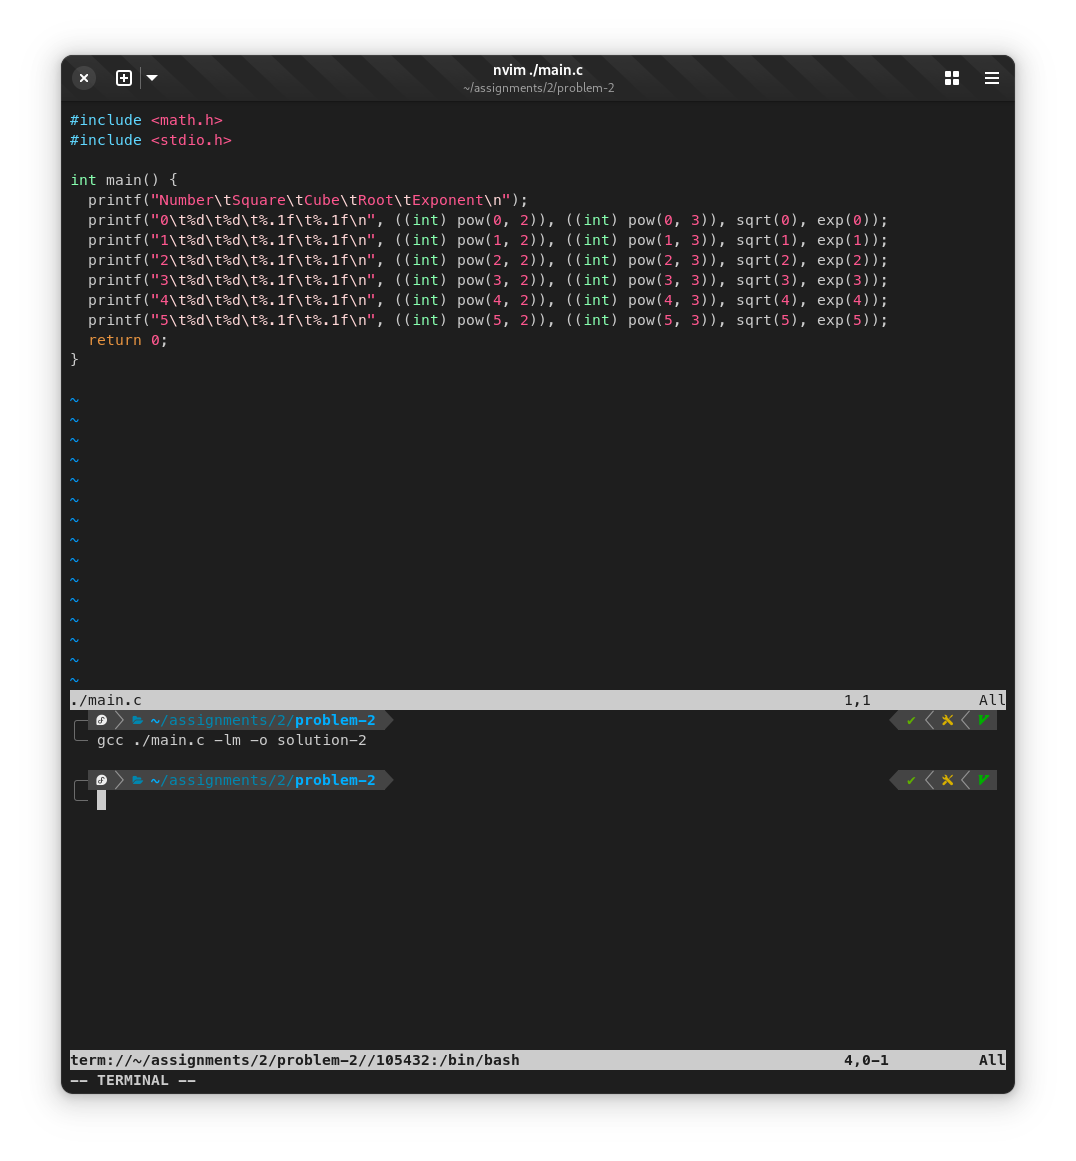
\includegraphics[width=1\linewidth,center]{src-2.png}
\subparagraph{Close Up Output Console Screenshot\\}
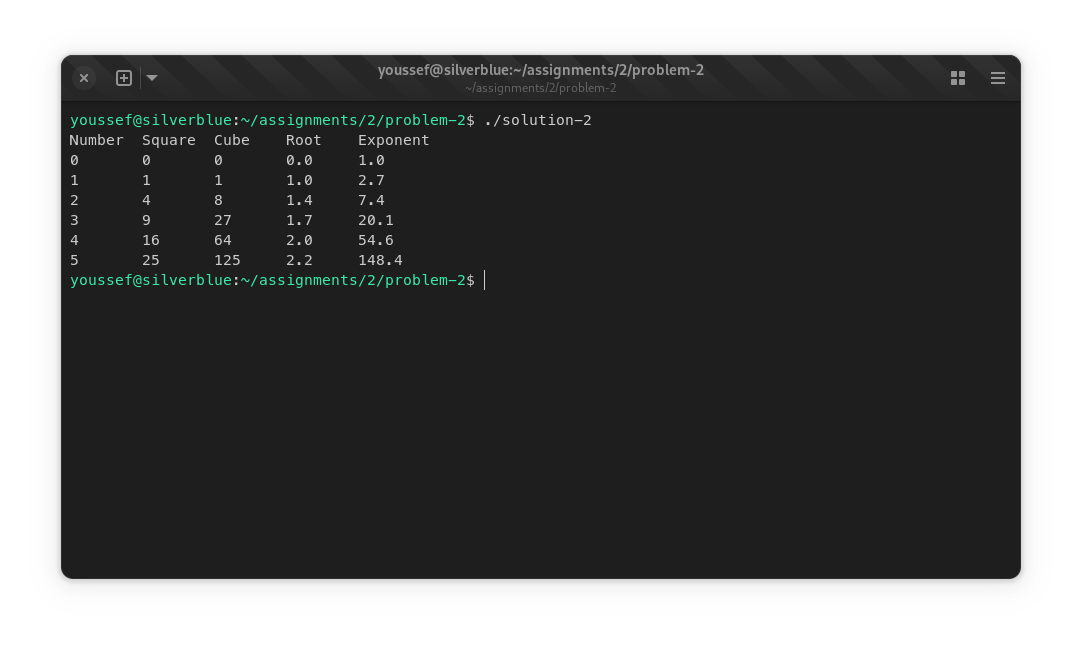
\includegraphics[width=1\linewidth,center]{out-2.png}
\subparagraph{Linux Desktop Screenshot\\\\}
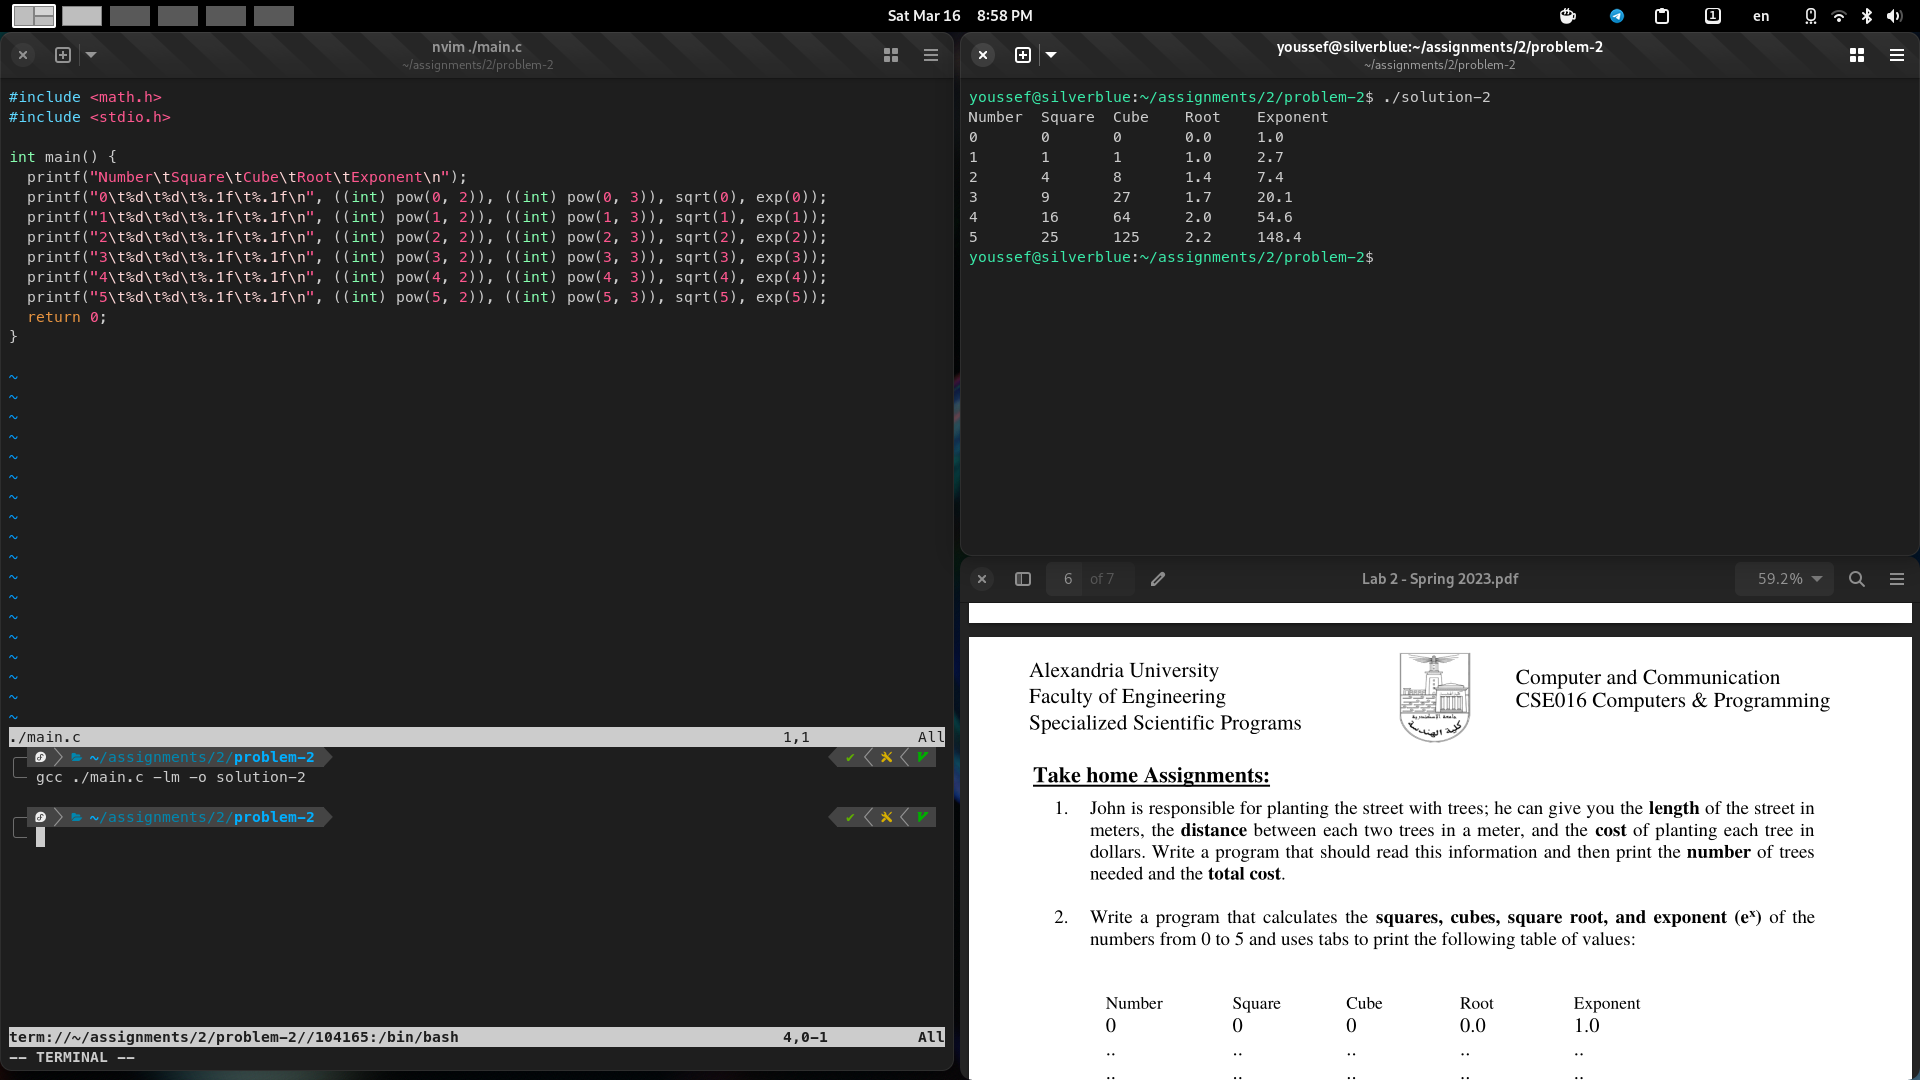
\includegraphics[width=1\linewidth,center]{desktop-2.png}
\newpage
\subsection{Specifications}
\begin{itemize}
    \item \textbf{Libraries:}
    \begin{itemize}
        \item \texttt{\color{inlinecode}{stdio.h}}
        \item \texttt{\color{inlinecode}{math.h}} 
    \end{itemize}
    \item \textbf{Compiler:} GNU C Compiler \texttt{\color{inlinecode}{(gcc)}} version 13.2.1 20231205 (Red Hat 13.2.1-6)
    \item \textbf{Supported Platforms:} OS: (any), architecture: (any)
    \item \textbf{Tested On:}
    \begin{itemize}
        \item Compiled on Fedora 39 Workstation Linux
        \item Ran on Fedora 39 Silverblue Workstation Linux
    \end{itemize}
\end{itemize}
\section{Licenses \& Warranty}
The software \& source code included are licensed under the BSD 3-Clause Open Source License: https://opensource.org/license/bsd-3-clause.\\\\
COPYRIGHT \copyright \ 2024, Youssef Ahmed Samy\\
Redistribution and use in source and binary forms, with or without modification, are permitted provided that the following conditions are met:

1. Redistributions of source code must retain the above copyright notice, this list of conditions and the following disclaimer.\\

2. Redistributions in binary form must reproduce the above copyright notice, this list of conditions and the following disclaimer in the documentation and/or other materials provided with the distribution.\\

3. Neither the name of the copyright holder nor the names of its contributors may be used to endorse or promote products derived from this software without specific prior written permission.
\\\\
THIS SOFTWARE IS PROVIDED BY THE COPYRIGHT HOLDERS AND CONTRIBUTORS “AS IS” AND ANY EXPRESS OR IMPLIED WARRANTIES, INCLUDING, BUT NOT LIMITED TO, THE IMPLIED WARRANTIES OF MERCHANTABILITY AND FITNESS FOR A PARTICULAR PURPOSE ARE DISCLAIMED. IN NO EVENT SHALL THE COPYRIGHT HOLDER OR CONTRIBUTORS BE LIABLE FOR ANY DIRECT, INDIRECT, INCIDENTAL, SPECIAL, EXEMPLARY, OR CONSEQUENTIAL DAMAGES (INCLUDING, BUT NOT LIMITED TO, PROCUREMENT OF SUBSTITUTE GOODS OR SERVICES; LOSS OF USE, DATA, OR PROFITS; OR BUSINESS INTERRUPTION) HOWEVER CAUSED AND ON ANY THEORY OF LIABILITY, WHETHER IN CONTRACT, STRICT LIABILITY, OR TORT (INCLUDING NEGLIGENCE OR OTHERWISE) ARISING IN ANY WAY OUT OF THE USE OF THIS SOFTWARE, EVEN IF ADVISED OF THE POSSIBILITY OF SUCH DAMAGE.
\newpage
\end{document}
